\documentclass{article}
\usepackage{graphicx} % Required for inserting images
\usepackage[colorlinks=true, linkcolor=blue, urlcolor=blue, framecolor=blue]{hyperref} % Customize link and box colors
\usepackage{float}
\usepackage{amsmath}

% Adjust page margins
\usepackage[margin=1in]{geometry} % Adjust the margin size as needed

\title{Dataset on Energy Consumption of Fischertechnik Quality Control}
\author{Aaditya Neupane}
\date{June 2025}

\begin{document}

\maketitle

\section{Dataset Overview}

This dataset contains detailed energy consumption measurements from the \textbf{Fischertechnik Quality \\ Control.} The data was collected at 100hz, 400hz, and 800hz sampling rates. For each sampling rate, 4000 experimental runs was done where colored Tabs (\texttt{Nio}, \texttt{Bio}, \texttt{Wio}, and \texttt{Rio}) were sorted by the system. Each experimental run generated a separate CSV file containing time-series measurements of electrical parameters.

\section{Experimental Setup}

\subsection{Physical System Components}

\begin{itemize}
  \item \textbf{Fischertechnik Quality Control (9v):} An industrial training model that simulates a real-world sorting system.
    \begin{figure}[h]
        \centering
        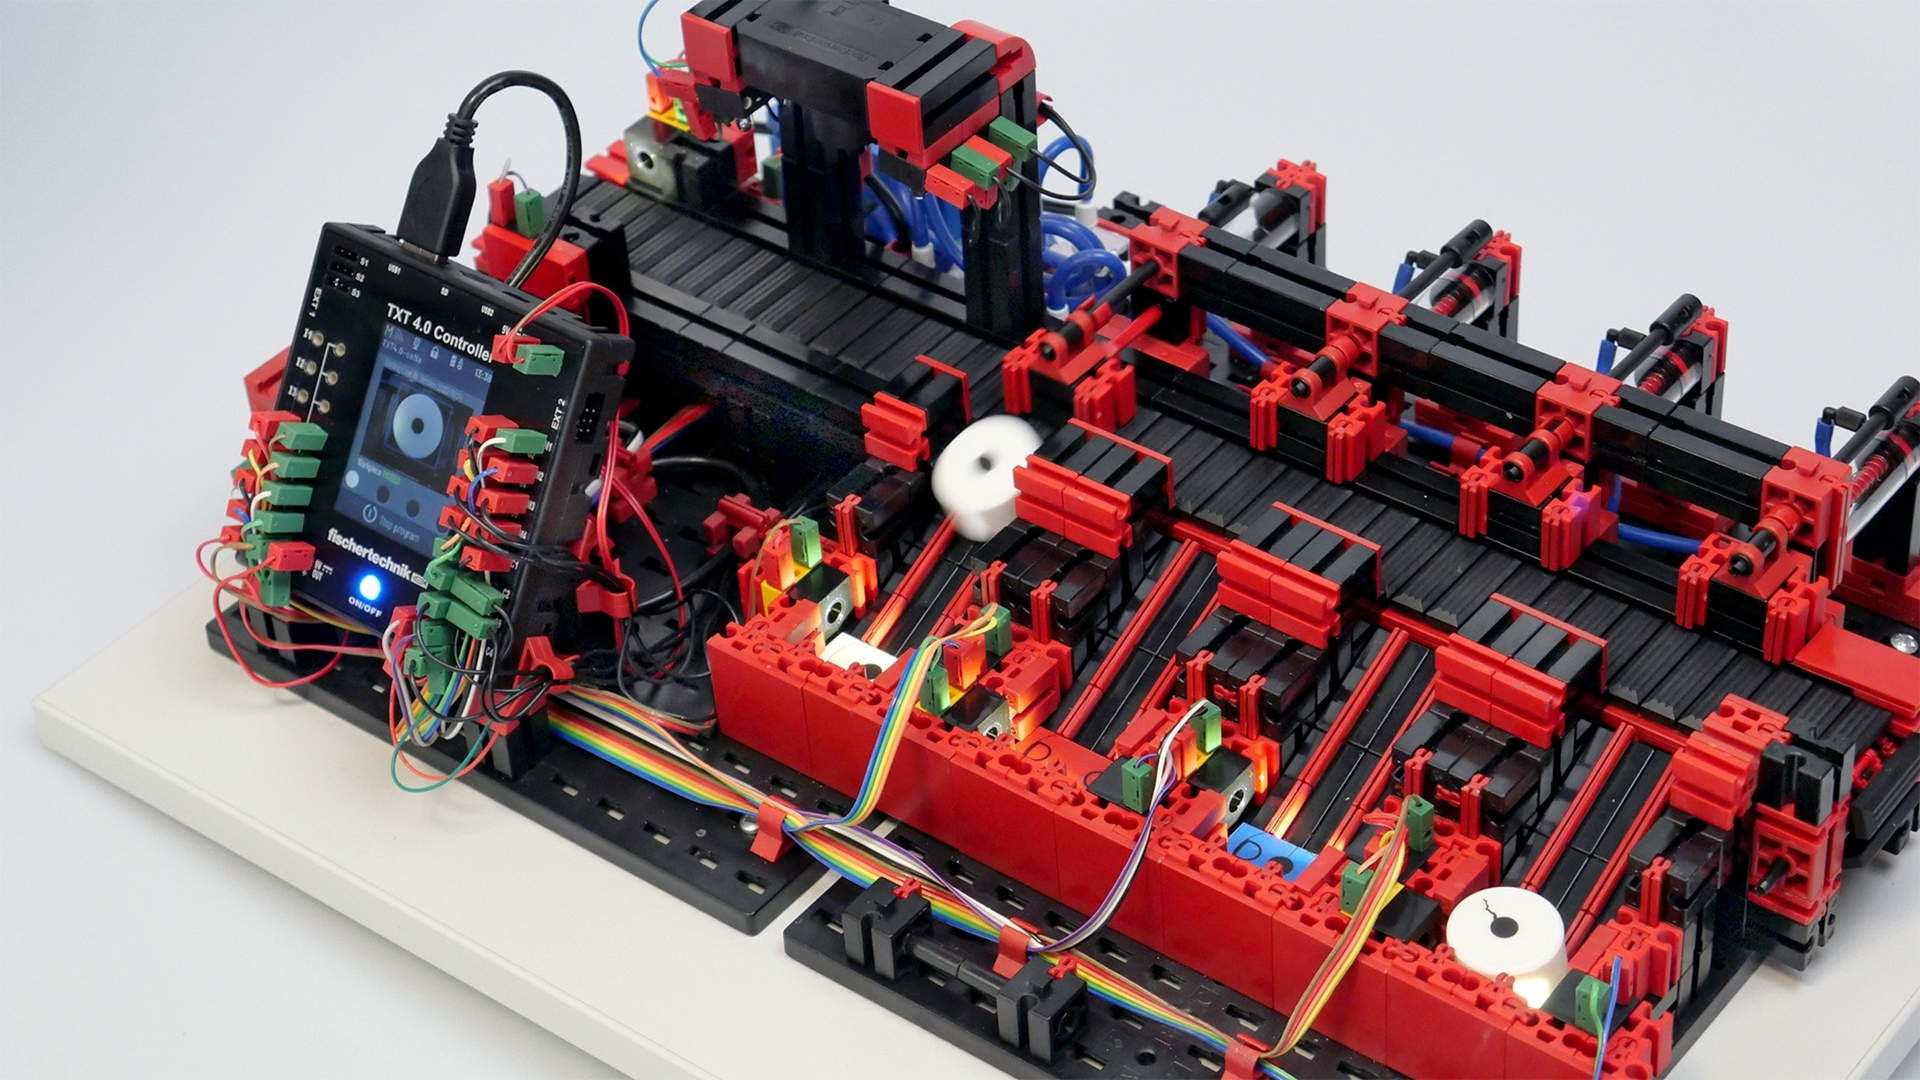
\includegraphics[width=0.4\linewidth]{quality_control.jpeg}
        \caption{Fischertechnik Quality Control}
        \label{fig:labels}
    \end{figure}



  
    \begin{itemize}
          \item \textbf{Vision System:} Includes a camera for Tab identification.
          \item \textbf{Conveyor Belt:} Transports Tabs from the starting point to the end point of the conveyor belt.
          \item \textbf{Pneumatic cylinders:} Pushes the Tabs on conveyor belt to the sorting destination.
          \item \textbf{Phototransistors:} At the starting point and at the sorting destination to start/stop conveyor belt.
    \end{itemize}
  \item \textbf{Power Supply:} Supplies 12v DC
  \item \textbf{DC to DC Converter:} Converts 12v DC to 9v DC
  \item \textbf{Arduino UNO:} Connected to a computer; it starts recording the electrical parameters from 'DC to DC Converter' when a Tab is detected by Phototransistor at starting point until it reaches (detected by Phototransistor) at sorting destination.
  \\
  \vspace{0.8cm}
  \\
  \item \textbf{Tabs:} \texttt{Nio}, \texttt{Bio}, \texttt{Wio}, and \texttt{Rio}
    \begin{figure}[h]
        \centering
        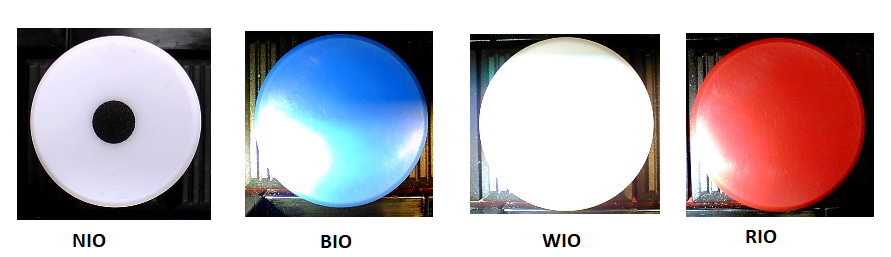
\includegraphics[width=1\linewidth]{objects.png}
        \caption{Tabs}
        \label{fig:labels}
    \end{figure}

\end{itemize}

\subsection{Data Collection Methodology}

\begin{itemize}
  \item \textbf{Trigger Mechanism:} Data recording begins when a Tab is placed at the starting point and stops when it reaches the sorting destination.
  \item \textbf{Sampling Frequencies:} Data is collected at 100\,Hz, 400\,Hz, and 800\,Hz
  \item \textbf{Repetition:} Each Tab was processed 1,000 times (4 Tab types × 1,000 runs = 4,000 datasets) for each sampling frequency.
  \item \textbf{Automatic File Generation:} Each sorting operation generates a separate CSV file.
\end{itemize}

\section{Data Description}

\subsection{File Structure}

\begin{itemize}
 

  \item \textbf{File Naming Convention:} \texttt{[Frequency]Hz\_Sort\_[Tab-Type-Name]\_[Date]\_[Count].csv} 
  \\
  example: \texttt{400Hz\_Sort\_biO\_06092024\_404.csv}
\item \textbf{Total Files:} 1000 files per Tab type for each sampling frequency = 1000 x 4 x 3 = 12,000 files
\item \textbf{Directory Structure}
\begin{figure}[h]
    \centering
    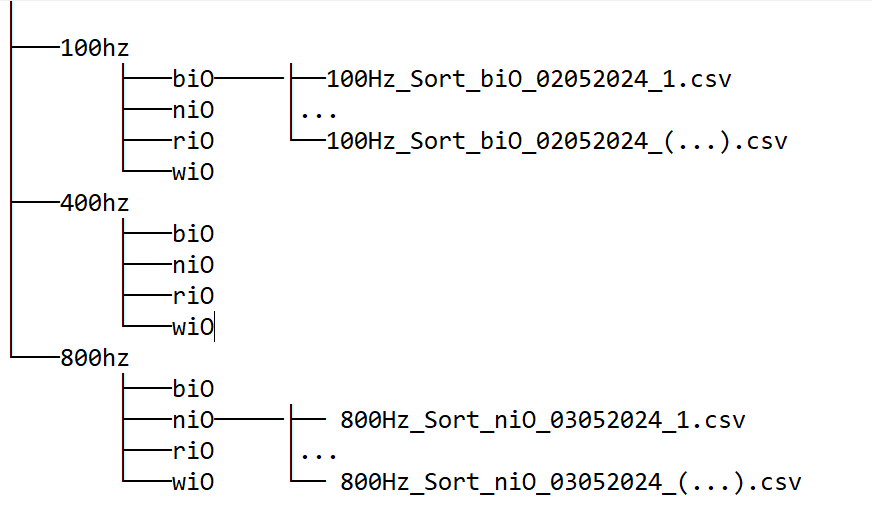
\includegraphics[width=0.5\linewidth]{file_structure.png}
    \caption{Directory Stucture}
    \label{fig:enter-label}
\end{figure}




  \item \textbf{File Organization:} Separated by Sampling frequency and by Tab types.
\end{itemize}

\subsection{Data Columns}

\begin{itemize}
  \item \texttt{Datum}: Date of recording (format: MM/DD/YYYY)
  \item \texttt{Uhrzeit}: Timestamp with microsecond precision (format: YYYY-MM-DD HH:MM:SS.microseconds)
  \item \texttt{I\_In (A)}: Input current in Amperes
  \item \texttt{V\_In (V)}: Input voltage in Volts
  \item \texttt{P\_In (W)}: Input power in Watts (calculated as V\_In × I\_In)
  \item \texttt{I\_Out (A)}: Output current in Amperes
  \item \texttt{V\_Out (V)}: Output voltage in Volts
  \item \texttt{P\_Out (W)}: Output power in Watts (calculated as V\_Out × I\_Out)
  \item \texttt{Temp (°C)}: System temperature of Arduino Uno in Celsius
  \item \texttt{Energie\_In (Wh)}: Cumulative input energy in Watt-hours 
  \item \texttt{Energie\_Out (Wh)}: Cumulative output energy in Watt-hours
  \\
    \noindent\hspace*{3.2cm}Calculated as:
\[
\Delta E = P \times \Delta t
\]
\[
E_{\text{new}} = E_{\text{previous}} + \Delta E
\]
\end{itemize}

\subsection{Measurement Characteristics}

\begin{itemize}
  \item Each file represents one complete sorting operation from start to finish.
  \item Various sampling frequencies (100hz, 400hz, 800hz)
  \item Synchronized and Standardized measurements across all 12,000 runs.
  \item Includes both instantaneous and cumulative measurements
  \item Timestamps with Microsecond Precision for time-series analysis
  \item Includes natural variations from repeated operations
\end{itemize}

\section{Potential Research Applications}

\begin{itemize}
  \item \textbf{Energy Efficiency Analysis:} Study power consumption patterns during sorting operations.
  \item \textbf{Machine Learning:} Develop models to predict Tab types/colors based on Energy Consumption data.
  \item \textbf{Process Optimization:} Identify inefficiencies in the sorting process.
  \item \textbf{Frequency Impact Analysis:} Examine how the sampling rate affects the performance of the ML models.
  \item \textbf{Anomaly Detection:} Identify unusual power consumption patterns that may indicate system issues.
\end{itemize}



\end{document}

